\documentclass[12pt,letterpaper]{article}
\usepackage{apa_manual}
\apatituloCorto{Teoría econométrica de las revisiones}

\begin{document}

\apacabecera
  {Econometría de las revisiones del PBI: noticias, ruido, sesgo, persistencia y no linealidad}
  {Manual teórico y práctico 4 — Fundamento estadístico de las Etapas 1 y 2}
  {Antes de entrenar modelos de Machine Learning o simuladores cuánticos debemos responder una pregunta económica elemental: ¿las correcciones que publica el BCRP obedecen a patrones sistemáticos observables en tiempo real o son meras sorpresas imposibles de anticipar? Este manual desarrolla el marco econométrico de las Etapas~1 y~2 y demuestra con pruebas robustas que existe estructura predecible —pero también quiebres de régimen y no linealidad pandémica— en las revisiones del PBI peruano.}

\section{La disyuntiva central de Mankiw y Shapiro: ¿noticias o ruido?}

Cuando una estadística oficial cambia entre su primera publicación \(y_t^{(v_0)}\) y una versión posterior \(y_t^{(v_H)}\), la revisión \(Y_t^{(H)} = y_t^{(v_H)} - y_t^{(v_0)}\) puede originarse por dos mecanismos económicos diametralmente opuestos \parencite{mankiw1986, croushore2011}. Distinguirlos no es un ejercicio académico menor: define si el problema de predicción tiene solución o si es teóricamente imposible superar el pronóstico cero.

\subsection{Hipótesis de Noticias (News)}

Bajo la hipótesis de \emph{noticias}, la agencia estadística actúa como un pronosticador racional perfecto: publica \(y_t^{(v_0)} = \mathbb{E}[y_t^{(v_H)} \mid \Omega_{v_0(t)}]\) utilizando de manera óptima toda la información \(\Omega_{v_0(t)}\) disponible en el momento de la primera nota. En consecuencia, las correcciones posteriores responden exclusivamente a información nueva (encuestas tardías, balances anuales, registros aduaneros o tributarios) que aún no existía cuando salió \(v_0(t)\):
\begin{equation}
  y_t^{(v_H)} = y_t^{(v_0)} + \nu_t, \qquad \mathbb{E}\bigl[Y_t^{(H)} \mid \Omega_{v_0(t)}\bigr] = 0, \qquad \text{Cov}\bigl(Y_t^{(H)},\, y_t^{(v_0)}\bigr) = 0.
  \label{eq:news}
\end{equation}
Una implicación algebraica directa es que la varianza de la cifra revisada excede a la de la primera estimación (\(\text{Var}(y_t^{(v_H)}) = \text{Var}(y_t^{(v_0)}) + \text{Var}(\nu_t) > \text{Var}(y_t^{(v_0)})\)). Si las revisiones del PBI peruano fueran pura noticia impredecible, ningún modelo alimentado con datos observables en \(v_0(t)\) podría derrotar sistemáticamente al pronóstico trivial \(\widehat{Y}_t^{(H)} = 0\).

\subsection{Hipótesis de Ruido o Sesgo Sistemático (Noise)}

Bajo la hipótesis opuesta de \emph{ruido}, la cifra definitiva ya está sujeta a una perturbación inicial de medición \(\eta_t\) incorporada en la primera lectura: \(y_t^{(v_0)} = y_t^{(v_H)} + \eta_t\), donde \(\eta_t\) es independiente del verdadero crecimiento revisado \(y_t^{(v_H)}\). Entonces la revisión futura \(Y_t^{(H)} = -\eta_t\) resulta negativamente correlacionada con la cifra inicial \(y_t^{(v_0)}\) (las estimaciones preliminares extremas tienden a moderarse hacia la media) y se invierte la desigualdad de varianzas: \(\text{Var}(y_t^{(v_0)}) > \text{Var}(y_t^{(v_H)})\).

Más allá del ruido puro de media cero, las agencias estadísticas suelen exhibir \textbf{sesgo direccional persistente} (por ejemplo, subestimar sectores dinámicos cuando las fuentes iniciales cubren empresas formales grandes y omiten temporalmente la actividad de medianas empresas o cosechas tardías) y \textbf{estacionalidad administrativa} en el calendario de cierre. En ese escenario híbrido —donde conviven noticias nuevas inevitables con sesgo sistemático, persistencia y errores de medición correlacionados con \(\Omega_{v_0(t)}\)— sí es legítimo y útil construir modelos predictivos en tiempo real.

\section{Horizonte limpio, colas pesadas e inferencia HAC (Newey--West)}

Como verificamos en la Etapa~1, las revisiones del PBI peruano no pueden analizarse sin separar antes los empalmes de año base (\codigo{2000m7} y \codigo{2014m3}). La Figura~\ref{fig:scatter_etapa2} confronta la primera estimación \(y_t^{(v_0)}\) frente al valor revisado once meses después \(y_t^{(v_{11})}\): los puntos limpios se agrupan ligeramente por encima de la línea de \(45^\circ\) (evidencia visual de sesgo positivo), mientras los \(24\) puntos afectados por cambio de base exhiben desviaciones artificiales severas hacia abajo.

\begin{figure}[htbp]
  \caption{Relación directa entre la primera estimación \(y_t^{(v_0)}\) y la estimación a \(H=11\) meses}
  \label{fig:scatter_etapa2}
  \centering
  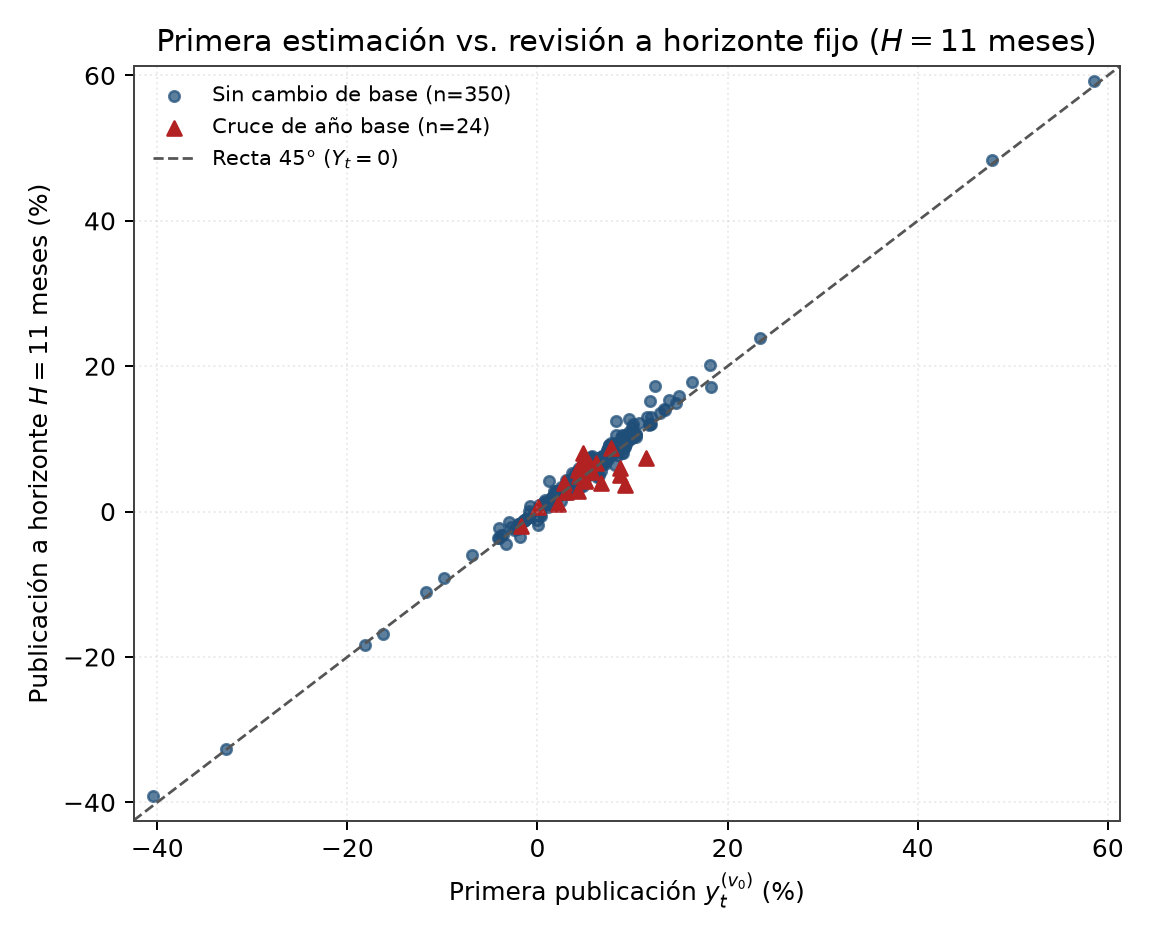
\includegraphics[width=0.80\textwidth]{figuras/scatter_revisiones_gdp.png}
  \apanota{Elaboración verificada sobre \codigo{muestra\_objetivo\_gdp.csv}. Se destacan por separado los \(24\) cruces de año base excluidos del núcleo analítico.}
\end{figure}

La Tabla~\ref{tab:horiz_etapa2} presenta los momentos estadísticos y pruebas formales sobre las muestras limpias de los horizontes \(H \in \{3, 6, 9, 10, 11, 12\}\), junto con la referencia bruta a \(H=11\). Dos resultados resaltan inmediatamente: primero, la media de revisión es positiva en todos los horizontes y crece monótonamente desde \(+0{,}205\) p.p. a tres meses hasta \(+0{,}347\) p.p. a \(H=11\) y \(+0{,}363\) p.p. a \(H=12\); segundo, retirar los \(24\) cruces de año base reduce el mínimo extremo de \(-5{,}500\) a \(-2{,}000\) p.p. y la desviación estándar de \(0{,}930\) a \(0{,}768\) p.p., evitando contaminar las pruebas con cambios contables.

\begin{table}[htbp]
  \caption{Diagnósticos descriptivos y pruebas HAC de sesgo medio según horizonte \(H\)}
  \label{tab:horiz_etapa2}
  \centering
  \setlength{\tabcolsep}{3.5pt}
  \begin{tabular}{@{}l S[table-format=3.0] S[table-format=1.3] S[table-format=1.3] l S[table-format=1.3] S[table-format=1.3] S[table-format=-1.3] S[table-format=1.1]@{}}
    \toprule
    Muestra & {$n$} & {Media} & {$\text{SE}_{\text{NW}}$} & {\(p_{\text{NW}}\)} & {DE} & {Mediana} & {Asim.} & {Curt.\ exc.} \\
    \midrule
    \(H=3\) limpia  & 358 & 0.205 & 0.033 & \(3{,}9\times 10^{-10}\) & 0.452 & 0.100 & 1.394 & 5.7 \\
    \(H=6\) limpia  & 355 & 0.311 & 0.047 & \(3{,}1\times 10^{-11}\) & 0.598 & 0.200 & 1.163 & 6.5 \\
    \(H=9\) limpia  & 352 & 0.335 & 0.057 & \(3{,}1\times 10^{-9}\)  & 0.690 & 0.200 & 0.906 & 4.7 \\
    \(H=11\) limpia & 350 & 0.347 & 0.064 & \(5{,}3\times 10^{-8}\)  & 0.768 & 0.200 & 1.258 & 6.3 \\
    \(H=11\) bruta  & 374 & 0.305 & 0.079 & \(1{,}1\times 10^{-4}\)  & 0.930 & 0.200 & -0.480 & 8.5 \\
    \(H=12\) limpia & 331 & 0.363 & 0.067 & \(5{,}7\times 10^{-8}\)  & 0.798 & 0.200 & 1.145 & 5.5 \\
    \bottomrule
  \end{tabular}
  \apanota{Datos de \codigo{output/etapa2\_econometria/etapa2\_descriptivos\_horizontes.csv}. Para \(H=11\) limpia, el estadístico de Jarque--Bera alcanza \(649{,}6\) (\(p=8{,}6\times 10^{-142}\)) y Shapiro--Wilk \(W=0{,}890\) (\(p=3{,}4\times 10^{-15}\)).}
\end{table}

\subsection{Por qué necesitamos errores estándar Newey--West (HAC)}

Para evaluar si la media muestral \(\bar{Y} = +0{,}347\) p.p. difiere significativamente de cero, sería erróneo aplicar el error estándar elemental \(s / \sqrt{n} = 0{,}768 / \sqrt{350} = 0{,}041\). ¿Por qué? Porque las revisiones \(Y_t^{(11)}\) y \(Y_{t+1}^{(11)}\) comparten diez meses calendario de historia estadística común; es decir, el solapamiento de ventanas de \(11\) meses induce autocorrelación serial positiva entre observaciones vecinas. Si ignoráramos esa dependencia positiva, subestimaríamos la varianza real del estimador y obtendríamos falsos positivos.

El estimador consistente ante heterocedasticidad y autocorrelación (HAC) de \textcite{newey1987} corrige esta dependencia sumando las autocovarianzas muestrales \(\hat{\gamma}_j\) ponderadas mediante el núcleo triangular de Bartlett, que garantiza que la varianza estimada nunca sea negativa:
\begin{equation}
  \widehat{V}_{\text{NW}}(\bar{Y}) = \frac{1}{n}\left[ \hat{\gamma}_0 + 2 \sum_{j=1}^{L} \left(1 - \frac{j}{L+1}\right)\hat{\gamma}_j \right].
  \label{eq:nw}
\end{equation}
En la Etapa~2 verificamos la robustez del contraste bajo dos elecciones del ancho de banda \(L\): la regla automática estándar \(L_{\text{NW}} = \lfloor 4(n/100)^{2/9} \rfloor = 5\) (\(\text{SE}_{\text{NW}} = 0{,}0638\), \(p = 5{,}3\times 10^{-8}\)) y una ventana conservadora ampliada hasta todo el horizonte de solapamiento \(L = H = 11\) (\(\text{SE}_{\text{solap}} = 0{,}0749\), \(p = 3{,}6\times 10^{-6}\)). Bajo ambos criterios, la hipótesis nula de media cero queda categóricamente rechazada.

\begin{figure}[htbp]
  \caption{Distribución empírica de las revisiones limpias \(Y_t^{(11)}\) y desplazamiento positivo respecto a cero}
  \label{fig:hist_etapa2}
  \centering
  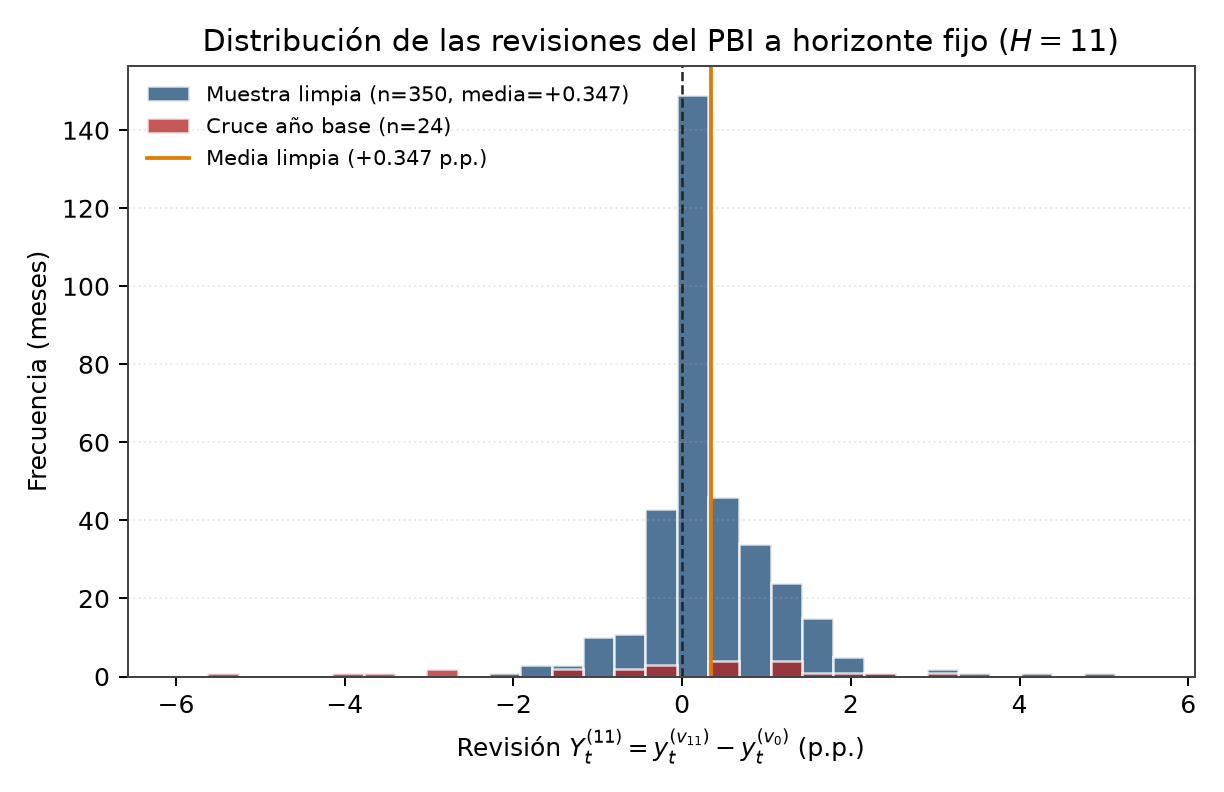
\includegraphics[width=0.84\textwidth]{figuras/hist_revisiones_gdp.png}
  \apanota{Tomado de la auditoría y caracterización de Etapas~1 y~2. Nótese la concentración asimétrica hacia valores positivos (\(+0{,}2\) p.p. de mediana; máximo limpio \(+4{,}9\) p.p.).}
\end{figure}

Adicionalmente, la Figura~\ref{fig:hist_etapa2} y la Tabla~\ref{tab:horiz_etapa2} revelan una marcada **no normalidad con colas pesadas**: la asimetría positiva (\(1{,}258\)) y el exceso de curtosis (\(6{,}293\)) rechazan la distribución gaussiana con \(p < 10^{-100}\) en la prueba de Jarque--Bera. Más aún, las pruebas de heterocedasticidad condicional autorregresiva (ARCH) de \textcite{engle1982} aplicadas a los residuos de \(Y_t^{(11)}\) son altamente significativas en orden \(1\) (\(p = 3{,}1\times 10^{-7}\)) y orden \(4\) (\(p = 1{,}1\times 10^{-5}\)), demostrando agrupamiento de volatilidad: las revisiones grandes tienden a concentrarse en épocas turbulentas. Esta evidencia justifica diseñar la Etapa~6 con innovaciones de colas pesadas (\(t_5 + \text{ARCH}\)) y explica por qué el error cuadrático medio (RMSE) castiga con tanta dureza los errores grandes aislados.

\section{Eficiencia de Mincer--Zarnowitz, regímenes históricos y prueba RESET}

Para contrastar de manera conjunta la racionalidad de la primera publicación frente a los dos mecanismos de Mankiw--Shapiro, estimamos la regresión clásica de \textcite{mincer1969}:
\begin{equation}
  y_t^{(v_{11})} = \alpha + \beta\, y_t^{(v_0)} + \varepsilon_t,
  \label{eq:mz}
\end{equation}
bajo la hipótesis nula conjunta \(H_0: \alpha = 0,\; \beta = 1\). Si el intercepto \(\hat{\alpha}\) difiere de cero, el anuncio inicial arrastra un sesgo constante corregible. Si la pendiente \(\hat{\beta}\) difiere de la unidad (especialmente \(\hat{\beta} < 1\)), las cifras iniciales extremas sobrerreaccionan y contienen ruido de medición que se corrige hacia la media.

En la muestra limpia global (\(n=350\)), obtenemos \(\hat{\alpha} = +0{,}2732\) (\(\text{SE}_{\text{NW}} = 0{,}0636\), \(p = 1{,}7\times 10^{-5}\)) y \(\hat{\beta} = 1{,}0175\) (\(\text{SE}_{\text{NW}} = 0{,}0095\), sin rechazo claro de \(\beta=1\) a \(5\%\): \(p = 0{,}068\)), con un \(R^2 = 0{,}9873\) y un rechazo contundente de la hipótesis conjunta de eficiencia (prueba de Wald HAC \(F = 16{,}234\), \(p = 1{,}8\times 10^{-7}\)). En términos intuitivos: la primera cifra del BCRP sigue casi uno a uno los movimientos de la cifra revisada (\(\beta \approx 1\)), pero parte sistemáticamente desplazada hacia abajo en casi tres décimas de punto porcentual (\(\hat{\alpha} > 0\)).

\subsection{Disociación por regímenes y significado de la prueba RESET}

¿Ese comportamiento lineal se mantuvo estable a lo largo de treinta años, o cambió tras las reformas estadísticas y la pandemia? Para averiguarlo, aplicamos en cada subperíodo tanto Mincer--Zarnowitz como la prueba RESET de \textcite{ramsey1969}, que añade potencias de los valores ajustados \((\hat{y}_t^2, \hat{y}_t^3)\) a la regresión lineal para comprobar si existe curvatura o no linealidad no capturada por una recta. Los resultados de la Tabla~\ref{tab:hallazgos_etapa2} y de la Figura~\ref{fig:regimenes_etapa2} revelan una historia económica sumamente nítida.

\begin{table}[htbp]
  \caption{Resumen econométrico por regímenes históricos en \(Y_t^{(11)}\) (Etapa~2)}
  \label{tab:hallazgos_etapa2}
  \centering
  \begin{tabular}{@{}p{4.8cm} S[table-format=3.0] S[table-format=1.3] S[table-format=1.3] S[table-format=1.3] l l@{}}
    \toprule
    Régimen histórico & {$n$} & {Media} & {DE} & {\(\hat{\beta}_{\text{MZ}}\)} & {Wald \(p_{\text{NW}}\)} & {RESET \(p\)} \\
    \midrule
    1993m10--1999m4 (Base 1990/94) & 67  & 0.633 & 1.289 & 1.052 & \(0{,}0125\)            & \(0{,}0514\) \\
    2000m6--2012m12 (Base 1994)    & 151 & 0.328 & 0.716 & 1.052 & \(5{,}8\times 10^{-5}\) & \(0{,}9112\) \\
    2014m2--2019m12 (Base 2007 pre-COVID) & 71 & 0.163 & 0.196 & 0.994 & \(1{,}0\times 10^{-6}\) & \(0{,}2085\) \\
    2020m1--2024m11 (COVID y post-COVID) & 59 & 0.305 & 0.371 & 1.004 & \(1{,}2\times 10^{-5}\) & \(0{,}00030\) \\
    \midrule
    \textbf{Muestra limpia global} & 350 & 0.347 & 0.768 & 1.018 & \(1{,}8\times 10^{-7}\) & \(0{,}00096\) \\
    \bottomrule
  \end{tabular}
  \apanota{Datos consolidados de \codigo{output/etapa2\_econometria/etapa2\_mincer\_zarnowitz.csv} y \codigo{etapa2\_regimenes\_y11.csv}.}
\end{table}

\begin{figure}[htbp]
  \caption{Evolución temporal por regímenes de las revisiones limpias \(Y_t^{(11)}\) (1993--2024)}
  \label{fig:regimenes_etapa2}
  \centering
  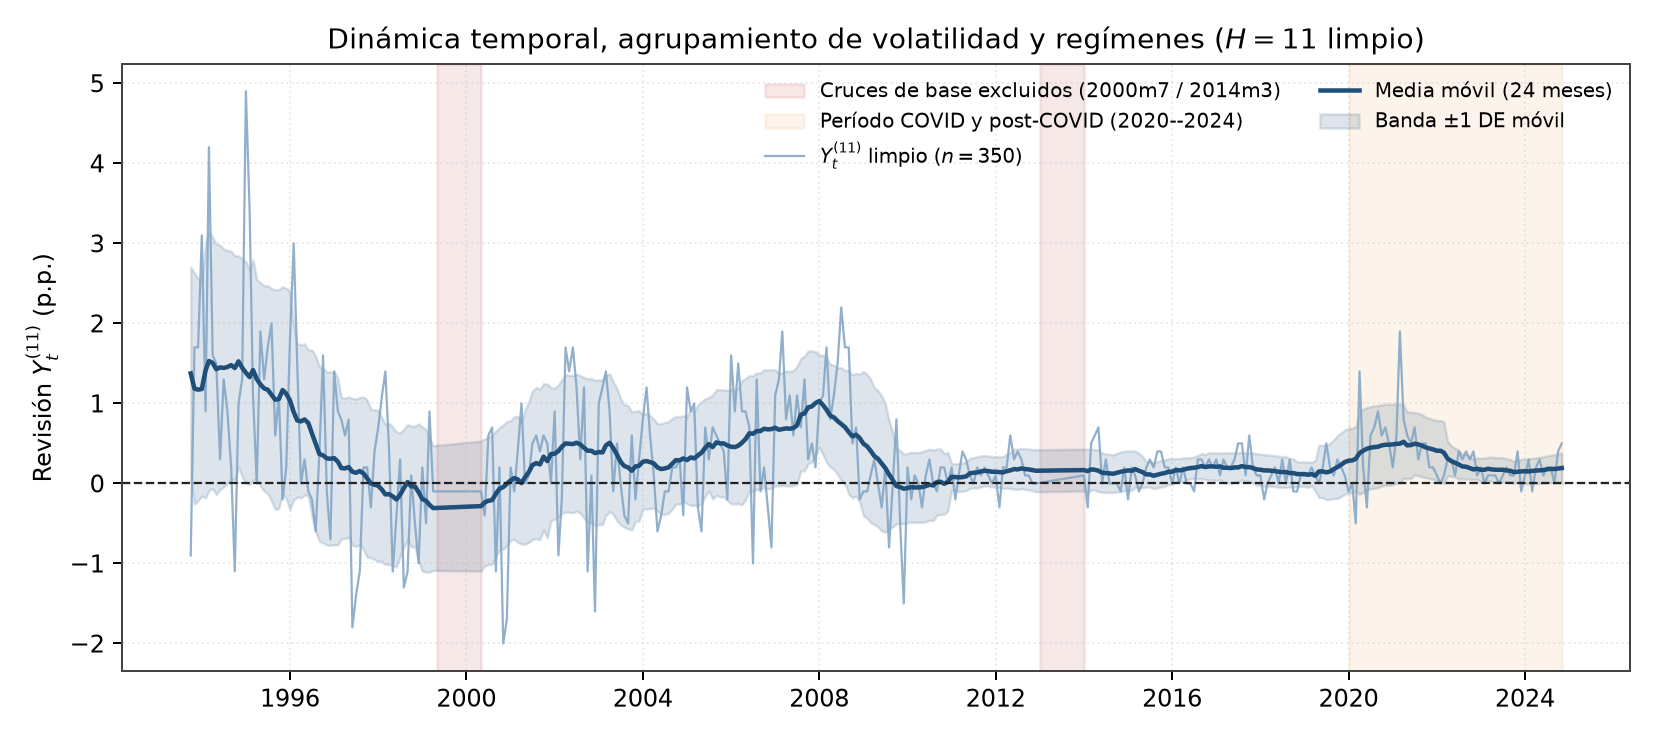
\includegraphics[width=0.92\textwidth]{figuras/etapa2_regimenes_evolucion.png}
  \apanota{Salida directa de \codigo{scripts/etapa2\_caracterizacion\_econometrica.py}. Se aprecia la moderación drástica de dispersión tras el cambio de año base de 2014 y el repunte en 2020.}
\end{figure}

Observa dos lecciones cruciales en la Tabla~\ref{tab:hallazgos_etapa2}:
\begin{enumerate}
  \item \textbf{Moderación gradual del sesgo y la volatilidad:} en los años noventa las revisiones promediaron \(+0{,}633\) p.p. con una desviación estándar de \(1{,}289\) p.p.; tras el cambio de base de 2000 bajaron a \(+0{,}328\) p.p. (\(\text{DE}=0{,}716\)), y tras la modernización estadística de base 2007 (2014--2019) se comprimieron a apenas \(+0{,}163\) p.p. (\(\text{DE}=0{,}196\)). Por ello, un modelo que promedie ciegamente toda la historia antigua sobreestimará el sesgo reciente.
  \item \textbf{La no linealidad está concentrada en el COVID-19:} antes de 2020, la prueba RESET \textbf{no rechaza la linealidad en ninguno de los tres regímenes previos} (\(p = 0{,}051\), \(0{,}911\) y \(0{,}208\)). Sin embargo, durante 2020--2024 el estadístico RESET se dispara a \(F = 9{,}439\) (\(p = 0{,}00030\)), arrastrando el resultado global a \(p = 0{,}00096\). Esto anticipa matemáticamente lo que veremos en la Etapa~3: en épocas normales una recta funciona muy bien, pero bajo choques extremos (\(y_0 = -40{,}5\%\) o \(+58{,}5\%\)) la relación lineal colapsa.
\end{enumerate}

\section{Frontera de observabilidad en tiempo real, estacionalidad y sectores}

Para diseñar modelos predictivos válidos, no basta con comprobar que la serie está autocorrelacionada; hay que preguntar \emph{qué rezagos están realmente terminados cuando se publica \(v_0(t)\)}. En efecto, la prueba global de \textcite{ljung1978} arroja \(Q(12) = 225{,}885\) (\(p = 1{,}4\times 10^{-41}\)), con autocorrelaciones muy altas en los primeros meses (\(\hat{\rho}_1 = +0{,}453\), \(\hat{\rho}_2 = +0{,}310\)). Sin embargo, como \(v_0(t) \approx t + 2\) meses y \(v_{11}(s) \approx s + 13\) meses, en el instante \(v_0(t)\) las revisiones acumuladas a \(11\) meses de \(t-1, t-2, \dots, t-10\) \textbf{todavía están en curso} y no existen en el mundo real.

\begin{figure}[htbp]
  \caption{Autocorrelación frente a la frontera de observabilidad en \(v_0\) (izquierda) y estacionalidad mensual (derecha)}
  \label{fig:acf_etapa2}
  \centering
  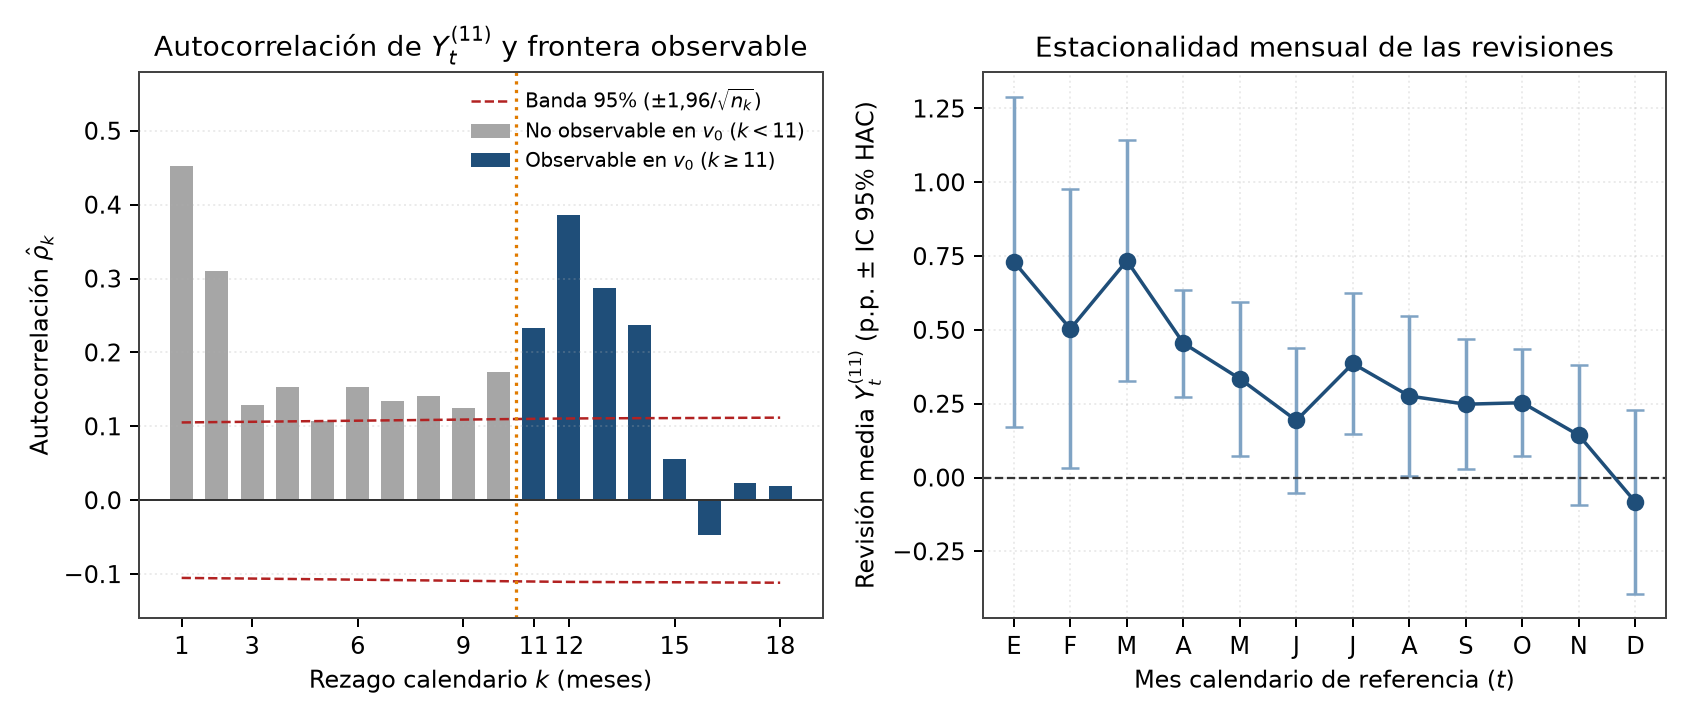
\includegraphics[width=0.95\textwidth]{figuras/etapa2_acf_pacf.png}
  \apanota{Tomado de \codigo{output/etapa2\_econometria/figures/etapa2\_acf\_pacf.png}. Solo los rezagos \(k \ge 11\) (a la derecha de la frontera vertical) son utilizables sin fuga temporal.}
\end{figure}

La Figura~\ref{fig:acf_etapa2} demuestra un hallazgo sobresaliente más allá de esa frontera (\(k \ge 11\)): reaparece un pico anual robusto exactamente en los rezagos observables \(\hat{\rho}_{11} = +0{,}234\) (\(p = 2{,}7\times 10^{-5}\)), \(\hat{\rho}_{12} = +0{,}386\) (\(p = 1{,}3\times 10^{-12}\), con autocorrelación parcial \(\hat{\phi}_{12,12} = +0{,}261\)) y \(\hat{\rho}_{13} = +0{,}288\) (\(p = 2{,}2\times 10^{-7}\)). En el panel derecho se observa además una estacionalidad marcada: los meses del primer trimestre sufren las mayores revisiones al alza (enero \(+0{,}731\), febrero \(+0{,}503\), marzo \(+0{,}734\) p.p.), descendiendo gradualmente hasta noviembre (\(+0{,}143\) p.p.) y diciembre (\(-0{,}083\) p.p.), probablemente por rezagos estacionales en reportes agrícolas y cierre de cuentas anuales.

Al combinar exclusivamente información observable en \(v_0(t)\) en una regresión diagnóstica (\(n=313\) observaciones completas en \codigo{etapa2\_asociacion\_tiempo\_real.csv}), los rezagos completados \(Y_{t-11}, Y_{t-12}\) explican por sí solos \(R^2 = 0{,}1569\) (\(F_{\text{NW}} = 9{,}197\), \(p = 0{,}00013\)), y la especificación conjunta con \(y_0\), rezagos anuales, revisiones tempranas de corto plazo (\(s=1,2\)) y estacionalidad alcanza \(R^2 = 0{,}2225\) (\(\bar{R}^2 = 0{,}1804\), \(F_{\text{NW}} = 4{,}190\), \(p = 2{,}6\times 10^{-7}\)).

\begin{figure}[htbp]
  \caption{Heterogeneidad sectorial del sesgo medio de revisión a horizonte \(H=11\) limpio}
  \label{fig:sectores_etapa2}
  \centering
  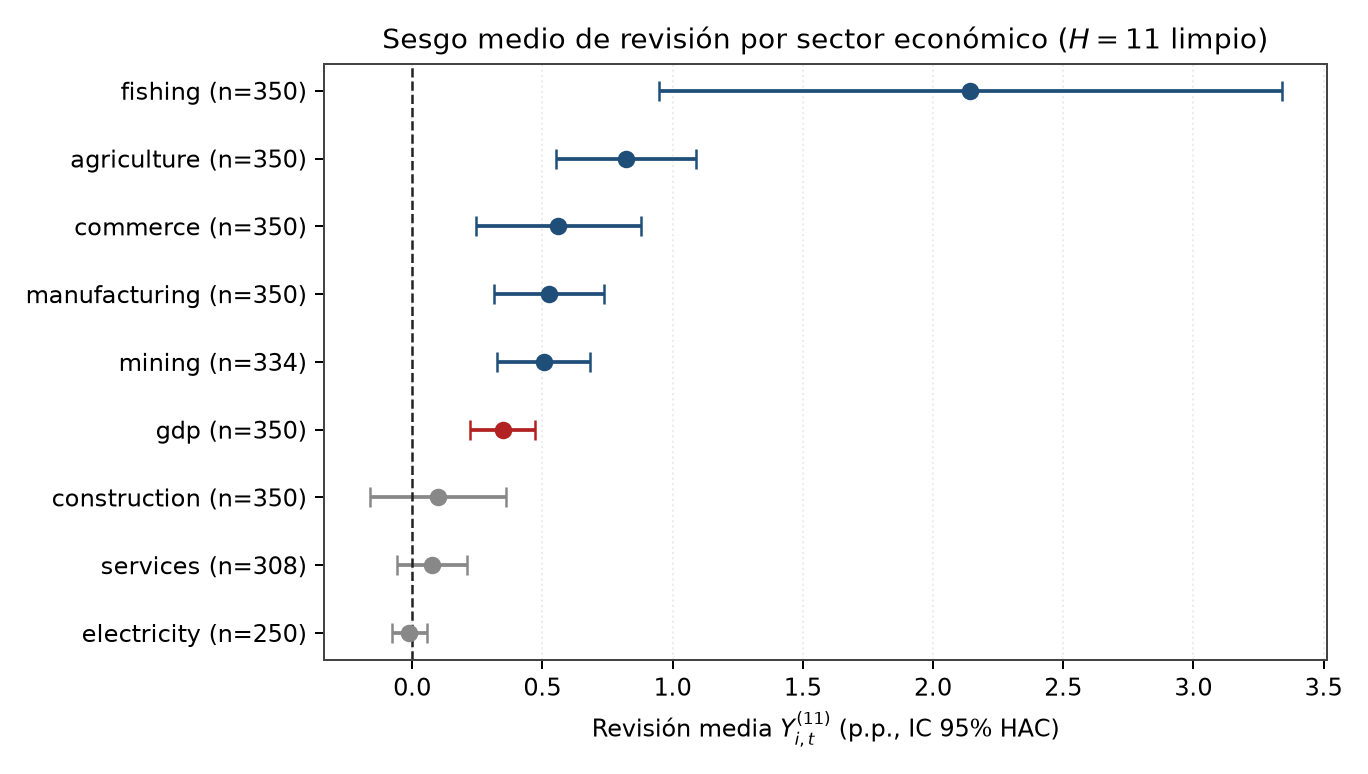
\includegraphics[width=0.84\textwidth]{figuras/etapa2_sectores_sesgo.png}
  \apanota{Datos de \codigo{output/etapa2\_econometria/etapa2\_sectores\_h11.csv} con intervalos de confianza al 95\% HAC/Newey--West.}
\end{figure}

Finalmente, la Figura~\ref{fig:sectores_etapa2} desagrega el origen productivo del sesgo agregado (\(+0{,}347\) p.p.). El fenómeno se concentra en sectores dependientes de encuestas de campo, extracción o comercio disperso: \textbf{pesca} (\(+2{,}143\) p.p., \(\text{DE}=7{,}448\), \(p=0{,}00045\)), \textbf{agropecuario} (\(+0{,}821\) p.p., \(p=2{,}1\times 10^{-9}\)), \textbf{comercio} (\(+0{,}562\) p.p., \(p=0{,}00052\)), \textbf{manufactura} (\(+0{,}525\) p.p., \(p=1{,}0\times 10^{-6}\)) y \textbf{minería e hidrocarburos} (\(+0{,}505\) p.p., \(p=3{,}0\times 10^{-8}\)). En contraste, \textbf{construcción} (\(+0{,}098\), \(p=0{,}462\)), \textbf{otros servicios} (\(+0{,}076\), \(p=0{,}273\)) y \textbf{electricidad y agua} (\(-0{,}011\), \(p=0{,}753\)), cuyas mediciones de despacho o facturación llegan casi en tiempo real, no muestran sesgo significativo respecto a cero.

\apabibliografia

\end{document}
